\documentclass{standalone}
\usepackage{tikz}
\usetikzlibrary{positioning,shapes,shadows,arrows}

\begin{document}
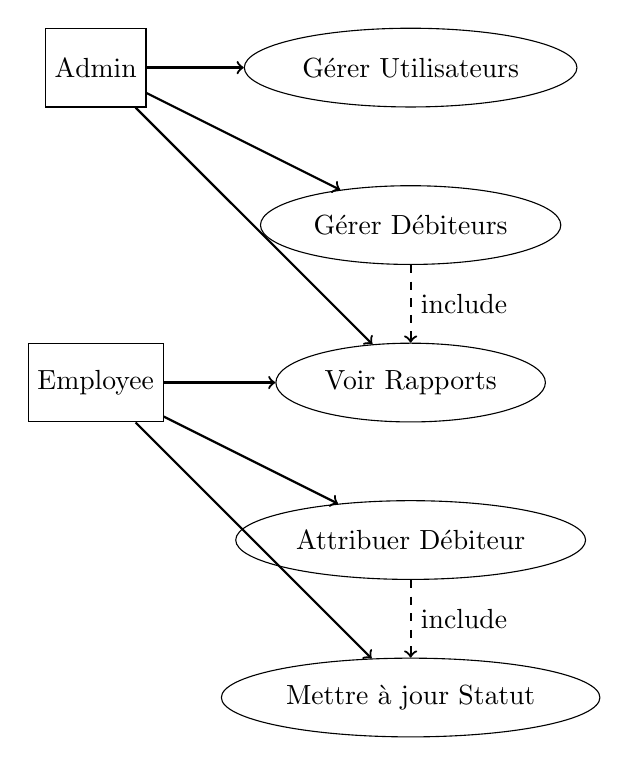
\begin{tikzpicture}[
    actor/.style={draw, minimum width=1cm, minimum height=1cm},
    usecase/.style={draw, ellipse, minimum width=2cm, minimum height=1cm},
    relation/.style={->, thick}
]

% Actors
\node[actor] (admin) at (0,0) {Admin};
\node[actor] (employee) at (0,-4) {Employee};

% Use Cases
\node[usecase] (manage_users) at (4,0) {Gérer Utilisateurs};
\node[usecase] (manage_debiteurs) at (4,-2) {Gérer Débiteurs};
\node[usecase] (view_reports) at (4,-4) {Voir Rapports};
\node[usecase] (assign_debiteur) at (4,-6) {Attribuer Débiteur};
\node[usecase] (update_status) at (4,-8) {Mettre à jour Statut};

% Relations
\draw[relation] (admin) -- (manage_users);
\draw[relation] (admin) -- (manage_debiteurs);
\draw[relation] (admin) -- (view_reports);
\draw[relation] (employee) -- (view_reports);
\draw[relation] (employee) -- (assign_debiteur);
\draw[relation] (employee) -- (update_status);

% Include relations
\draw[relation, dashed] (manage_debiteurs) -- node[right] {include} (view_reports);
\draw[relation, dashed] (assign_debiteur) -- node[right] {include} (update_status);

\end{tikzpicture}
\end{document} 